\documentclass[10pt]{article}
%\pagestyle{headings}

\oddsidemargin 0.0in
\evensidemargin 0.0in
\textwidth 6.0in
\topmargin 0.2in
\footskip 20pt
\textheight 8.5in

\usepackage{hyperref,color,graphicx,mathrsfs,amsmath,pdflscape,datetime}
\usepackage[numbers,sort]{natbib}
\hypersetup{colorlinks,%
            citecolor=blue,%
            linkcolor=blue,%
            filecolor=blue,%
            urlcolor=red}

\bibliographystyle{unsrtnat}
\renewcommand{\rmdefault}{phv}

	\begin{document}
{\noindent\Large{\textbf{Track reconstruction in NEXT with Deep Neural Networks (DNNs)}}}\\
Updated: \today\\ %, at \ampmtime \\

\noindent One of the most important aspects of the NEXT experiment is its ability to reconstruct the ionization tracks produced when energetic electrons deposit their
energy in the high pressure xenon gas present inside the NEXT detector.  Because many natural radioactive processes can produce energy depositions with an energy similar 
to that of neutrinoless double-beta decay,\footnote{For xenon, this energy is $Q_{\beta\beta} \approx 2.4$ MeV and common backgrounds include gamma rays produced by nuclear
decay of $^{208}$Tl and $^{214}$Bi.} and because neutrinoless double-beta decay is so rare, we will likely see many events in NEXT with energies that make them look like they could be
neutrinoless double-beta decay.  This will occur despite the shielding provided by the many meters of rock in the Pyrenees mountains, the lead castle inside which the detector is placed, and
the copper shielding inside the detector surrounding the active region!  These \textbf{background} events must be discarded (``rejected'') while the real double-beta events - the \textbf{signal} 
events - are kept.  By just looking at the energy deposited by each event, we will be able to remove many events that do not have the energy of interest, but at some point this no longer works
because all detectors have a finite energy resolution and we will have to choose a region of energies of potential interest.  Many background events will still fall into this region.\\

\noindent NEXT has further power to reject background because the ionization track of most background events (those due to gamma rays) will be produced by a single electron while the
track of a neutrinoless double beta ($0\nu\beta\beta$) event is produced by two electrons.  Because of the way energetic electrons lose energy in gaseous detectors, these two types of
ionization tracks will, most of the time, look distinctly different.  In particular, energetic electrons ionize xenon atoms at a lower density when they have higher energy, and the ionization density
increases as the electron loses energy.  Energetic electrons are also subject to less multiple scattering\footnote{Electron multiple scattering is the phenomenon responsible for
causing energetic electrons to undergo sudden sharp changes in direction while depositing their energy.} at higher energies than at lower energies.  Thus a single-electron track will look smoother
near the beginning with less energy deposited per unit distance, and more distorted near the end, with a ``blob'' of higher-density energy deposition at the end.  A track produced by two electrons
emitted from a common vertex (such as in $0\nu\beta\beta$) will be smoother and less dense near the vertex and have two such ``blobs'' at the ends.\\

\noindent In order to make use of this additional handle on background rejection, we must have a well-reconstructed track.  Our goal in this study will be to evaluate the performance of deep 
neural networks DNNs in reconstructing the $(x,y)$ coordinates of individual energy depositions in NEXT.

\section{Introduction: NEXT and particle track reconstruction}
\noindent NEXT reconstructs particle tracks, which are groups of ionization electrons liberated by interactions in the detector.  
Once this ionization track is produced, the
electrons are drifted to an amplification region in which each one is accelerated to the point at which it repeatedly excites atoms in the xenon medium over a narrow region
nominally 5 mm in width producing a number of photons proportional to the width of the region.  This process is called electroluminescence, and the narrow region in which light is
produced is called the electroluminescent gap (EL gap).  The basics of NEXT detector operation are explained schematically in Fig. \ref{fig_SS}.\\

\begin{figure}[!htb]
	\centering
	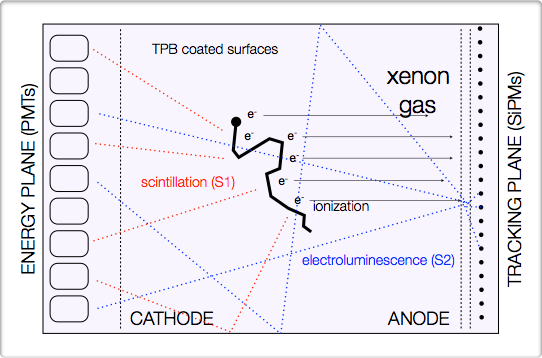
\includegraphics[width= 0.95\textwidth]{fig/nextEL.png}
	\caption{Principle of operation of NEXT.} \label{fig_SS}
\end{figure}

\noindent NEXT detectors contain two types of devices that observe the light produced by interactions in the detector.  A plane of photomultiplier tubes (PMTs) - which measures a relatively larger
fraction of the light produced - is called the ``energy plane'' and is located on the side of the detector opposite to the narrow light production region. A plane of silicon photomultipliers (SiPMs) is 
located next to the EL gap and is called the ``tracking plane''.  The S1 and S2 light produced by an event as measured by the energy plane give a ``waveform'' similar to that shown in figure 
\ref{fig_PMTwaveform}.\\

\begin{figure}[!htb]
	\centering
	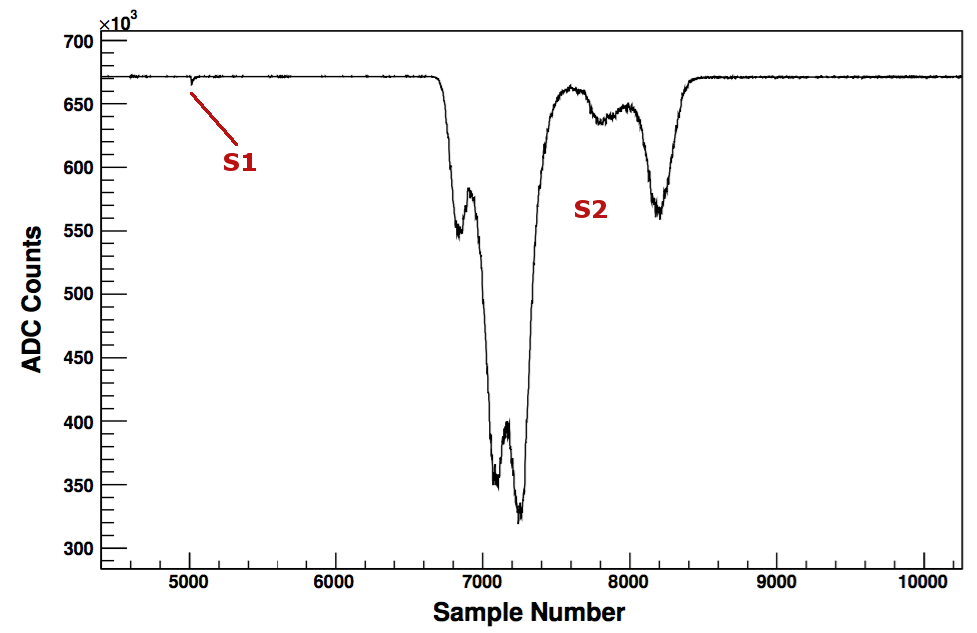
\includegraphics[width= 0.95\textwidth]{fig/example_PMT_waveform.png}
	\caption{A example of a waveform (sum over all PMTs) produced by the interaction of a 662 keV $\gamma$ ray in the NEXT-DBDM prototype detector.} \label{fig_PMTwaveform}
\end{figure}

\noindent Because the drift velocity of ionization electrons is well known in xenon gas, the difference in time between the ``S1'' light produced when the initial interaction occurs and the arrival of 
the corresponding ``S2'' light can be used to calculate the z-coordinate at which that
ionization electron was produced in the detector.  This is measured using the PMT (energy) plane, as a more precise measurement of the total light produced can be made by this plane than by
the SiPM (tracking) plane.  However, each SiPM should give a waveform similar to the one produced in the energy plane, but because the tracking plane is closer to the EL gap, the variations in the
amount of light detected by each SiPM are much greater (some are located much closer to the point at which the S2 light was produced than others).  Figure \ref{fig_PMTandSiPM} shows a muon event and the
corresponding waveforms measured in the energy plane and tracking plane.\\

\begin{figure}[!htb]
	\centering
	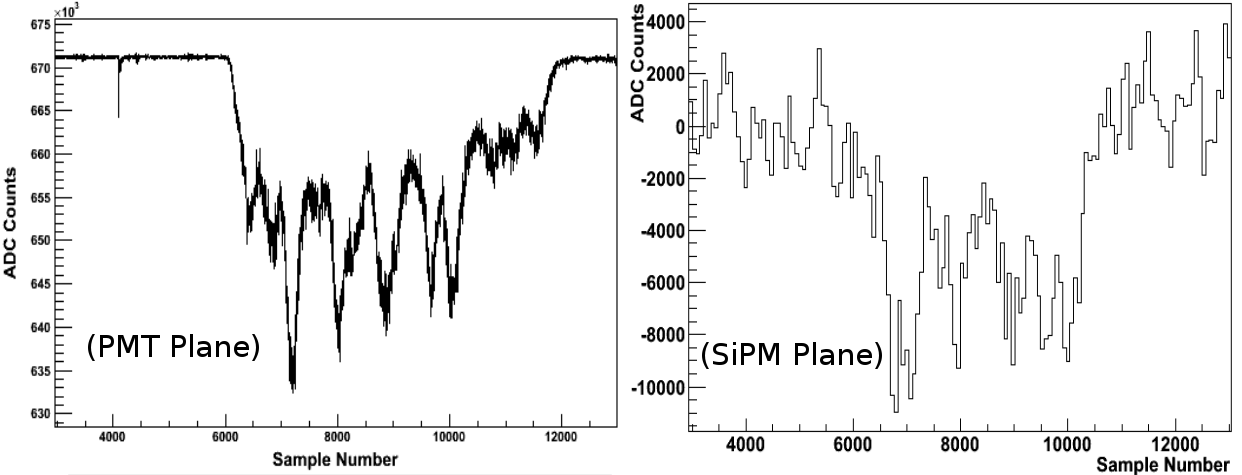
\includegraphics[width= 0.95\textwidth]{fig/c3_fig_sum_waveforms.png}
	\caption{A muon event measured in the PMT plane (left) and SiPM plane (right) in the NEXT-DBDM prototype detector.  In each case the sum over all individual PMTs/SiPMs is shown.}\label{fig_PMTandSiPM}
\end{figure}

\noindent The S2 signal for each event can be divided into slices, and for each slice the z-coordinate can be calculated using drift time and the (x,y) coordinates using the pattern of light on 
the SiPM plane.  Rather than coming up with a detailed algorithm to determine from the responses of each SiPM, we will attempt to train a ``deep neural network (DNN)'' to do the job for us.  Deep 
neural networks have been used to solve difficult problems such as recognizing handwritten characters and understanding human speech.  Ideally we would have a DNN that is properly trained so
that we can show it a response pattern on the tracking plane and it will tell us where the ionization electron was in (x,y).

\noindent Once the event has been divided into slices and the $(x,y,z)$ coordinates determined for each slice, space is then divided up into small rectangular volumes called ``voxels,'' and the energy from each slice is added into the voxel in which it is located.  Examples of the resulting reconstructed tracks are shown in figures \ref{fig_bgexample} and \ref{fig_siexample}.  
We currently expect to use 10x10x5 mm$^3$ voxels in NEXT, though events voxelized in 2x2x2 mm$^3$ voxels are displayed in the figures, as they better exhibit the details in the tracks.

\begin{figure}[!ht]
	\centering
	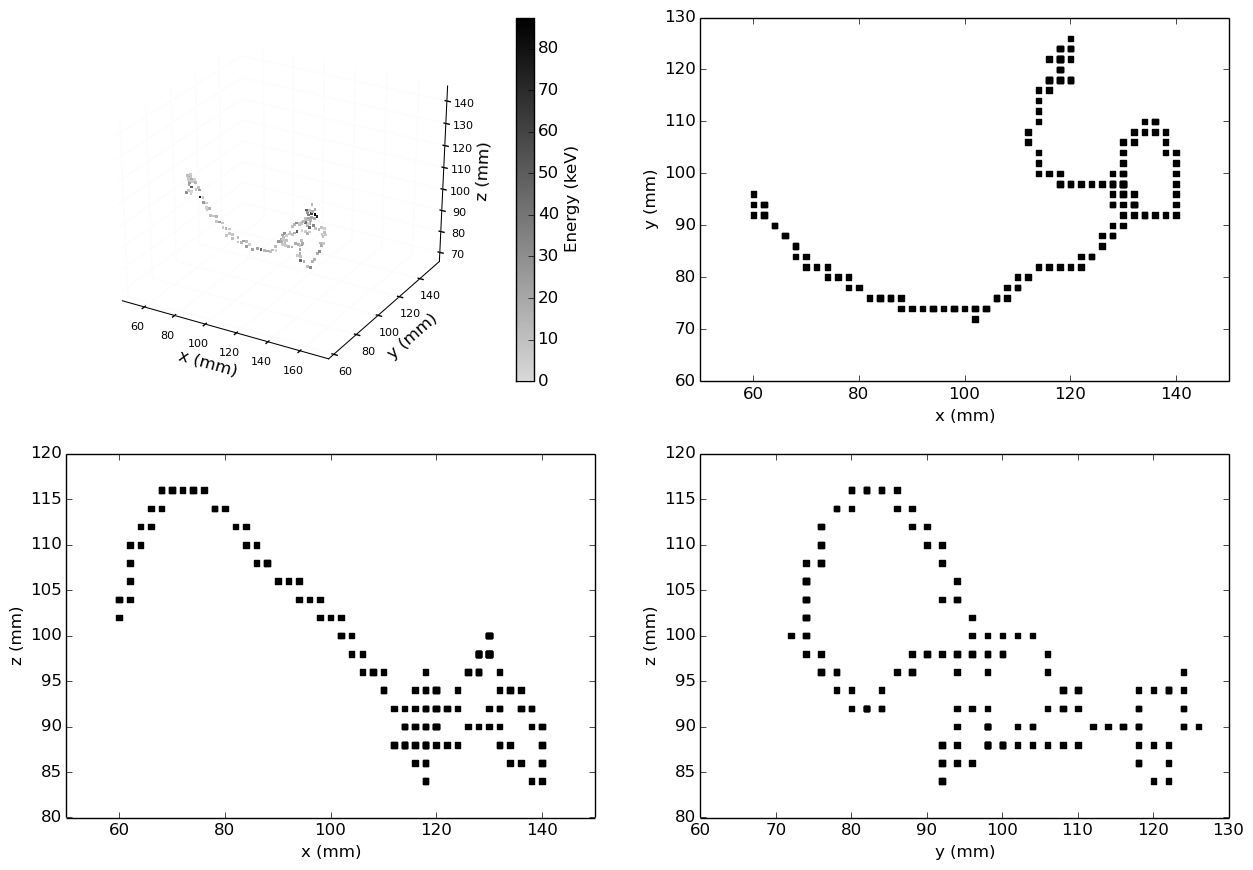
\includegraphics[scale=0.4]{fig/plt_dnn3d_NEXT100_Paolina222_v2x2x2_r200x200x200_bg_5.png}
	\caption{\label{fig_bgexample}Example of a simulated \textbf{background} event voxelized in volumes of 2x2x2 mm$^3$.}
\end{figure}

\begin{figure}[!ht]
	\centering
	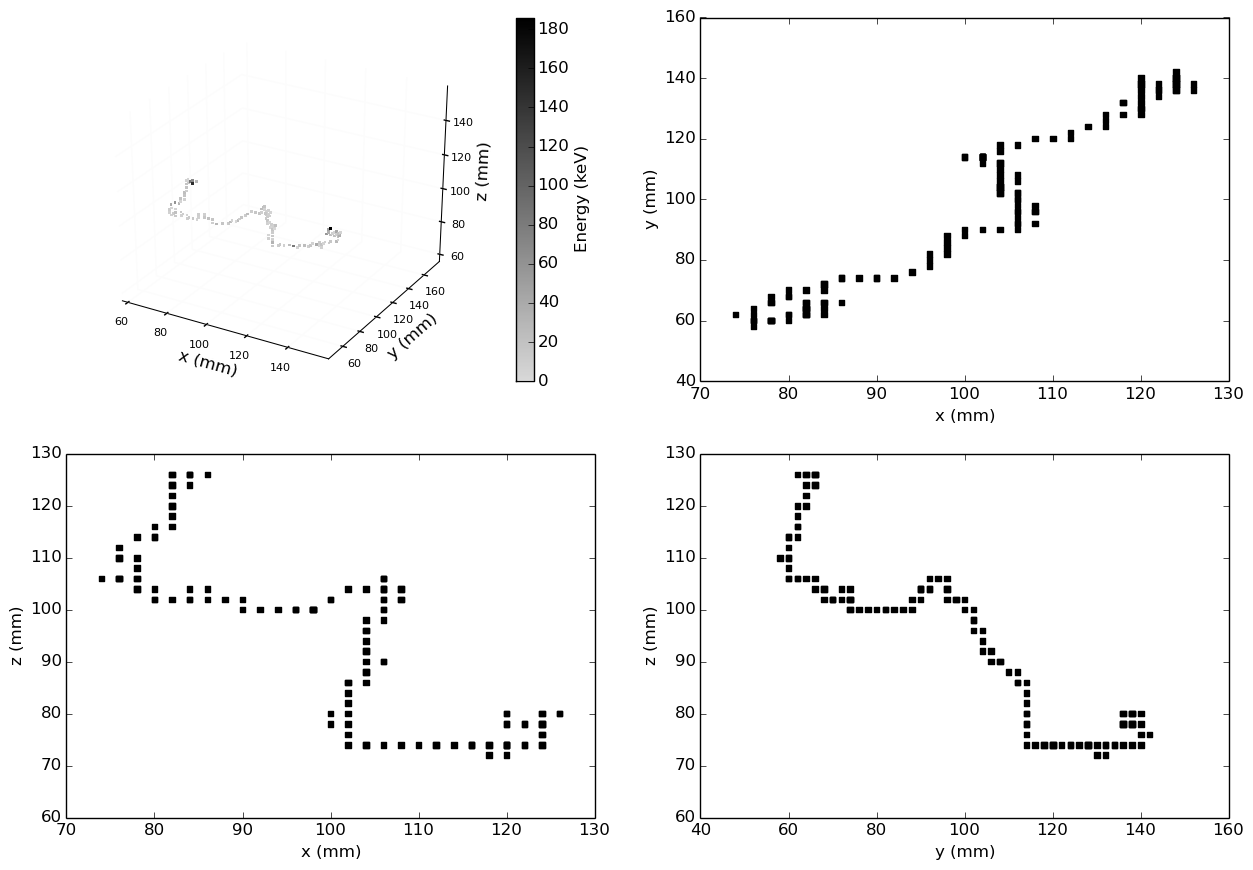
\includegraphics[scale=0.4]{fig/plt_dnn3d_NEXT100_Paolina222_v2x2x2_r200x200x200_si_2.png}
	\caption{\label{fig_siexample}Example of a simulated \textbf{signal} event voxelized in volumes of 2x2x2 mm$^3$.}
\end{figure}

\section{Energy loss of particles in matter}
\noindent When energetic particles such as the electrons produced in neutrinoless double-beta decay travel through matter, such as the high-pressure xenon detector medium of NEXT, they
slow down and eventually stop by transferring their energy to the atoms of the medium through excitations and ionizations.  This process is not the same for every particle and medium, and much
study has gone into understanding this (see for example the summary from the \href{http://pdg.lbl.gov/2014/reviews/rpp2014-rev-passage-particles-matter.pdf}{Particle Data Group}).\\

\noindent One of the most important characteristics of electron energy loss in xenon is the tendency for an energetic electron to deposit a large amount of energy in a small region at the end
of its track.  We will now do a calculation that will help in understanding this.\\

\subsection{Calculation: The ``Bragg Peak''}
\noindent Assume a particle moves through a medium with energy loss per unit length $dE/dx$ inversely proportional to the square of its velocity.  Assume also that the particle is 
non-relativistic so that its energy $E$ is proportional to the square of its velocity ($E = \frac{1}{2}mv^{2}$), so that

\begin{equation}
\frac{dE}{dx} = -\frac{k}{E}
\end{equation}

\noindent where $k$ is some constant.

\begin{enumerate}
	\item[1.] For initial particle energy $E_{i}$, what is the energy $E$ as a function of the distance traveled $x$?
	\item[2.] What is $dE/dx$ as a function of the distance traveled $x$?
	\item[3.] Plot $\frac{1}{E_i}|dE/dx|$ vs. $x$ for several values of $k/E_{i}^2$ (this can be done quickly with something like \href{https://www.wolframalpha.com/}{Wolfram Alpha} - for example to plot 
	x$^2$, just type in \verb|plot x^2|).  What do you notice about how the rate of energy loss $dE/dx$ changes as the distance traveled increases?  Note that at some
	point the energy of the particle becomes 0 and $dE/dx$ becomes infinite.  This is a result of our assumptions and would not happen in reality.
\end{enumerate}

\section{A Monte Carlo Simulation of SiPM Responses}
\subsection{Simulation Outline}
\noindent Rather than attempting to use the response of the SiPMs in the tracking plane for fully simulated events, we will instead make a smaller Monte Carlo simulation in ROOT.
In this case we can evaluate how well the DNN-based reconstruction will work using a simpler and controlled set of events - if it doesn't work under these conditions, it probably won't work in a 
more realistic case.  Let's consider an 8x8 plane of SiPMs, each with active area of 1 mm$^2$ and positioned with a pitch (distance between SiPMs) of 1 cm.  We assume we can only have
EL light (electroluminescent light, produced just in front of the SiPM plane) in a 9 cm x 9 cm area, and that this light is produced at a single point within that area.\\

\begin{figure}[!ht]
	\center
	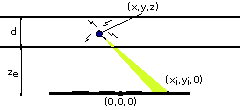
\includegraphics[scale=2.5]{fig/el_sipm_theory.pdf}
	\caption[A single EL electron emitting light instantaneously at a location $(x,y,z)$ in the EL gap]{\label{fig:el_sipm_theory}A single EL electron 
		emitting light instantaneously at a location $(x,y,z)$ in
		the EL gap.  A fraction of this light strikes the face of the SiPM located at $(x_{i},y_{i})$ on the SiPM plane.}
\end{figure}

\noindent EL light emitted from a single point (x,y) has some probability of hitting an SiPM, which we will label with an index $i$, located at $(x_i,y_i,z_i)$.  To calculate this probability we will
consider the setup shown in figure \ref{fig:el_sipm_theory}.  Consider the uniform emission of light from a point
$(x,y,z)$ in the EL gap, which has a width $d$ and ends a distance $z_e$ above the SiPM plane.  We now ask what fraction of the emitted light is incident on an SiPM of area 
$A = 1 \, \mathrm{mm}^2$ at location $(x_{i},y_{i},0)$ (see figure \ref{fig:el_sipm_theory}).  Assuming $z^{2} \gg A$ and the flux density a distance $r$ from the emission point is
$\mathbf{{I}} = (I_{0}/4\pi r^{2})\mathbf{\hat{r}}$, we have a flux at the SiPM face of 
$\mathbf{I} \cdot \mathbf{A}$, where $\mathbf{A} = A\mathbf{\hat{z}}$.  We consider the emission of a single photon and
interpret the quantity $\mathbf{I} \cdot \mathbf{A}/I_{0}$ as the probability of this photon striking the face of SiPM $i$.  Thus the probability
that a single photon emitted at $(x,y,z)$ will strike the face of the SiPM at $(x_{i},y_{i})$ is

\begin{equation}
p(x,y,z;x_{i},y_{i}) = \frac{A}{4\pi}\Biggl(\frac{z}{((x-x_{i})^{2} + (y-y_{i})^{2} + z^{2})^{3/2}}\Biggr),
\end{equation}

\noindent where we have used $\mathbf{\hat{r}}\cdot\mathbf{\hat{z}} = z/\sqrt{(x-x_{i})^{2} + (y-y_{i})^{2} + z^{2}}$.
For a given number of photons emitted uniformly over the EL gap, we average this probability over the interval
$z \in [z_{e},z_{e}+d]$

\begin{equation}\label{eqn_detprob}
\begin{split}
\bar{p}(x,y;x_{i},y_{i}) = & \frac{1}{d}\int_{z_{e}}^{z_{e}+d}p(x,y,z;x_{i},y_{i})dz\\
= & \frac{A}{4\pi d\sqrt{(x-x_{i})^{2}+(y-y_{i})^{2} + z_{e}^{2}}}\Biggl[1-\sqrt{\frac{(x-x_{i})^{2}+(y-y_{i})^{2}+z_{e}^{2}}{(x-x_{i})^{2}+(y-y_{i})^{2}+(z_{e}+d)^{2}}}\,\,\Biggr].
\end{split}
\end{equation}

\noindent Now we can write a Monte Carlo simulation by considering the following procedure:

\begin{enumerate}
	\item[1.] Choose a point $(x,y)$ on a grid with spacing $\delta$ in each direction.
	\item[2.] Calculate the probability of detecting a photon for each SiPM and thus generate a random number of photons detected by each SiPM (the ``SiPM response'').  Note that this will require choosing a number of
	photons to be emitted and will therefore require some information about the physics of the electroluminescence process.
	\item[3.] Normalize the array of SiPM responses to a mean of $\mu = 0$ and a standard deviation of $\sigma = 1$.
	\item[4.] Save the $(x,y)$ location of the point along with the generated SiPM response array in a ROOT tree.
\end{enumerate}

\noindent This will require:

\begin{enumerate}
	\item[-] A function which takes a number of generated photons at a location $(x,y)$ and calculates the response for an SiPM located at $(x_i,y_i)$ using equation \ref{eqn_detprob}
	\item[-] A function which steps over a grid of points, uses the above function to generate the response of each SiPM at each grid point, and saves the location of the grid point and 
	writes the responses of the SiPMs to a \verb|TTree|.
\end{enumerate}

\subsection{Adding Fluctuations to the SImulation}
\noindent Rather than simply computing the probability of detection for each sensor, we ultimately want to consider statistical fluctuations on the sensor responses.  Also, because the magnitude 
of the fluctuations will vary based on the number of photons detected, we want to compute a number of detected photons that would be suitable based on the number of photons used in NEXT
to reconstruct a single ``hit'' (energy deposition corresponding to a single SiPM map).\\

\noindent We will calculate the number of photons to be generated per SiPM map given the following information:

\begin{enumerate}
	\item[-] Each of our sensor maps will contain light produced due to the electroluminescence of ionization electrons produced during the creation of the particle track.  Assume that this light
	for a single sensor map represents between 30 keV and 150 keV of deposited energy.
	\item[-] The W-value, or the amount of energy necessary to create a single ionization electron in the track, is about $W_{i} = 25$ eV.
	\item[-] Each ionization electron will produce a number of photons $n$ during electroluminescence equal to
	
	\begin{equation}\label{eqn_ELgain}
	n = 140(E/p - 0.83)p\Delta x,
	\end{equation}
	
	\noindent where $E$ is the electric field applied in the electroluminescent region (in kV/cm), $p$ is the pressure of the xenon gas (in bar), and $\Delta x$ is the width of the EL gap (in cm).
\end{enumerate}

\noindent To find the number of photons contributing to each SiPM response map:

\begin{enumerate}
	\item[1.] Calculate the number of ionization electrons produced for a 30 keV and 150 keV energy deposition.
	\item[2.] Calculate the number of photons produced by a single ionization electron $n$ using equation \ref{eqn_ELgain} for $p = 15$, $E/p = 3$, and $\Delta x = 0.5$.
	\item[3.] Therefore calculate the range for $N$, the total number of photons produced (for a 30 keV energy deposition and for a 150 keV energy deposition).
\end{enumerate}

\noindent Now rather than each SiPM response being a detection probability $\bar{p}$ as calculated by equation \ref{eqn_detprob}, it should be a random number of photons 
generated with mean $N\bar{p}$ and variance $N\bar{p}(1-\bar{p})$.  If the mean $N\bar{p}$ is less than about 100, one can use the 
binomial distribution to generate the random number of photons.  Otherwise for mean greater than 100, the Gaussian distribution would give a good approximation.  We will pick $N$ to
be somewhere in the range calculated above.  ROOT has some methods such as \verb|Binomial| and \verb|Gaus| of the
\href{https://root.cern.ch/doc/master/classTRandom3.html}{TRandom3} class to generate random numbers.

\section{Deep Neural Networks (DNNs)}
\noindent We will now attempt to train a DNN to output the correct EL grid point when given a pattern of SiPM responses.  The DNN will have an input layer consisting of the 64 SiPM responses and
an output layer of 1600 neurons that yield the probability that each of the grid points is the correct point.  The DNN code is written in Python and uses the library
\href{https://www.tensorflow.org}{TensorFlow}.  In the \verb|dnntracks/dnn| directory there should be several Python files:

\begin{enumerate}
	\item[--] \verb|dnninputs.py|: used to define input parameters
	\item[--] \verb|dnntrain.py|: used to run the training based on the specified parameters
	\item[--] \verb|dnnplot.py|: used to make key plots of the data and results
\end{enumerate}

\noindent The structure of the DNN is described in the file \verb|nets/neuralnets.py|.  To run the DNN training:

\begin{enumerate}
	\item[1.] Run the SiPM response Monte Carlo in ROOT to generate a number of SiPM response maps for random EL points on the 1600-point grid.  10000 is a good number of events to start with.
	\item[2.] Move the .root file generated by the simulation to a location (for example, a new folder called \verb|data| in your user home directory), and set the variables correctly in the file
	\verb|dnninputs.py|.
	\item[3.] Run the training step\footnote{Note: running a Unix command followed by the amperstand \& will run that command in a separate Unix shell so you can continue issuing further commands without having to wait until it finishes.}: \verb|python dnntrain.py &|
	\item[4.] Once the training step finishes, plots of the results can be made using \verb|dnnplot.py|
\end{enumerate}

\appendix
\section{Overview of computing tools used}\label{ss_computingtools}
\noindent The following is a brief summary of the key tools to be used:

\begin{enumerate}
	\item[\textbullet] \textbf{\href{https://root.cern.ch}{ROOT}}: a data analysis code developed at CERN.
	\item[\textbullet] \textbf{Python}: much of the code we will run is written in Python.  With previous programming knowledge, 
	Python should be readable, and a quick search on the Internet will probably provide code for how to perform specific operations
	(such as reading/writing to a file, creating a multidimensional array ...) when in doubt.  It is a good idea to obtain some
	familiarity with the basics of the language, and for this, working through sections 1-4 of 
	\href{https://docs.python.org/2/tutorial/}{this Python tutorial} (or a similar one) would be helpful.  
%	Several widely-used Python libraries may be used including \href{http://matplotlib.org}{matplotlib}, \href{http://www.numpy.org}{numpy}, and \href{http://www.h5py.org}{h5py}.
	\item[\textbullet] \textbf{Linux}: the analysis will be done in a Linux environment.  In most cases the necessary commands
	will be mentioned in this document and some miscellaneous commands can be found in appendix \ref{s_app_linux}.  As
	the code and files that will be edited are stored on another machine accessed remotely, it will be helpful to become familiar
	with a text editor such as \href{https://www.gnu.org/software/emacs}{emacs}.
	\item[\textbullet] \textbf{\href{https://www.tensorflow.org}{TensorFlow}}: this is a Python library that facilitates the creation and 
	training of neural networks.  Another library based on C$++$ which we will not use is \href{http://caffe.berkeleyvision.org}{Caffe}.
	\item[\textbullet] \textbf{\href{https://git-scm.com}{git}}: a version control system that allows you to store, update, and share
	code with multiple people at the same time.  It is used when multiple people are working on the same project.  The basics of Git can be learned quickly from \href{https://try.github.io}{this online tutorial}.
\end{enumerate}

\section{Linux environment}\label{s_app_linux}
\noindent Mac OS supports Unix commands - just open the application ``Terminal'' and you can start issuing such commands.  A useful more powerful terminal for Mac OS is 
(\href{https://www.iterm2.com}{iTerm2}).  The discussion in this section does not apply to Windows, but Windows users can still connect to a Linux machine 
remotely via ssh.  For this one would need to download an ssh client such as \href{http://www.putty.org}{PuTTY}.

\subsection{ssh and scp}\label{ss_app_sshscp}
\noindent Two useful commands that can be used to communicate with other Linux/Unix machines are \verb|ssh| and \verb|scp|.  To connect to another machine using \verb|ssh|, use

\begin{verbatim}
 ssh -X user@machine.address
\end{verbatim}

\noindent where \verb|user| is the user name and \verb|machine.address| is the name and address of the machine to which to connect (for example, \verb|analysis01.ific.uv.es|).  Note that 
creating a new text file (named, for example \verb|analysis01|) and placing in it the above command, then issuing the command,

\begin{verbatim}
 chmod a+x analysis01
\end{verbatim}

\noindent the file becomes ``executable'' so that as a shortcut one can execute the ssh command just by running \verb|./analysis01|.\\

\noindent The \verb|scp| command allows one to transfer files to or from the specified machine.  For example, to transfer file \verb|datfile.txt| in the current directory of the current machine to the directory 
\verb|/home/user/data| on machine \verb|analysis01.ific.uv.es| via login \verb|user|,

\begin{verbatim}
 scp datfile.txt user@analysis01.ific.uv.es:/home/user/data
\end{verbatim}

\subsection{Some Unix commands}\label{ss_app_commands}
\noindent Here are some basic Unix commands.

\subsubsection{\texttt{cat}}
\noindent This command can be used to print the contents of a file to the terminal.  Example: 

\begin{verbatim}
  cat code.py
\end{verbatim}

\subsubsection{\texttt{cd}}
\noindent This command changes directories.  For example, if one wanted to change to the directory ``folder'' contained in the current directory one could type:

\begin{verbatim}
  cd folder
\end{verbatim}

\noindent Just typing \verb|cd| will take you straight to your ``home'' directory no matter what directory you are currently in.\\

\noindent The ``parent'' directory (the one containing the current directory) is represented by two dots \texttt{..} in Unix/Cygwin commands.  The following command will change directories to the parent directory.
\begin{verbatim}
  cd ..
\end{verbatim}
  
\subsubsection{\texttt{cp <file> <destination>}}
\noindent This command copies a file to the location specified (similar to \texttt{mv}, except the original file is kept).  To make a copy of ``data.c'' located in the directory src and name it ``old\_data.c'':

\begin{verbatim}
  cp data.h5 old_data.h5
\end{verbatim}

\subsubsection{\texttt{exit}}
\noindent This command is used to quit the current Linux terminal.

%\subsubsection{\texttt{gcc <source\_file.c> -o <out\_file>}}
%\noindent This command is used to compile a C program.  For example, to compile the file \texttt{source.c} into the program called \texttt{pgm}:
%
%\begin{verbatim}
%  gcc source.c -o pgm
%\end{verbatim}
      
\subsubsection{\texttt{ls}}
\noindent This command lists all the files in the current directory.

\subsubsection{\texttt{mkdir} \textless dir\textgreater}
\noindent This command creates a new directory specified by \textless dir\textgreater.  To create a directory called \texttt{folder} in the current directory:

\begin{verbatim}
  mkdir folder
\end{verbatim}
	  
\subsubsection{\texttt{mv <file> <destination>}}
\noindent This command moves a file to the specified location.  For example to move the file ``code.py'' into a directory called ``srcdir'' that is contained in the current directory:

\begin{verbatim}
  mv code.py srcdir
\end{verbatim}

\noindent You can also use \texttt{mv} to rename files.  To rename ``code.py''' to ``old\_code.py'':
\begin{verbatim}
  mv code.py old_code.py
\end{verbatim}

\noindent Note that you can also move and rename at the same time.  The following renames ``code.py'' to ``old\_code.py'' and moves it to directory called ``srcdir'':
\begin{verbatim}
  mv code.py srcdir/old_code.py
\end{verbatim}

\noindent Note that in \texttt{mv} and \texttt{cp} and other commands, the current directory is specified by (\texttt{.}) - a single dot.  To move ``code.py'' from the directory ``srcdir'' to the current directory:
\begin{verbatim}
  mv srcdir/code.py .
\end{verbatim}

\subsubsection{\texttt{kill <PID>}}
\noindent This command ends a process with ID \verb|<PID>|.  To view a list of running processes and process IDs, use the \verb|ps| command.  To kill all processes for a given program,
use \verb|killall <name>|, for example \verb|killall emacs|.

\section{Using git}
\noindent Once changes have been made, in the folder into which the git repository has been cloned, the changes can be sent to the repository by taking the following steps.\\

\noindent First, it is a good idea to download/merge any previous changes before trying to submit new ones:

\begin{verbatim}
git pull
\end{verbatim}

\noindent Now the changes to files in the repository can be viewed in addition to files that have been created but not yet added to the repository by using,

\begin{verbatim}
git status
\end{verbatim}

\noindent Then one can commit the changes that have been made and write a message describing them.  For example, to commit file1.C and file2.C,

\begin{verbatim}
git commit -m "Message describing changes" file1.C file2.C
\end{verbatim}

\noindent Once changes have been committed, use the ``push'' command to send them to the repository,

\begin{verbatim}
git push
\end{verbatim}

\section{Trees in ROOT}
\noindent To use the \verb|TTree| class in ROOT, one normally works in the following order:

\begin{enumerate}
 \item[1.] Create a \verb|TTree| object.
 \item[2.] Create branches for the tree and assign them to variables
 \item[3.] Fill the variables with the values that you want to store in the tree
 \item[4.] Write an ``event'' to the tree (fill the branches with the values in the variables)
 \item[5.] Repeat steps 3 and 4 for each event
\end{enumerate}

\noindent For example (see also for example \href{https://root.cern.ch/root/html/tutorials/tree/tree2.C.html}{this tutorial}):
\begin{verbatim}

  // Make a TFile in which to store the tree.
  TFile f("new_file.root");
  
  // Make the tree
  TTree * tr = new TTree("tree_name","tree_description");
  
  // Make the variables to be assigned to branches.
  int var1, var2;
  double var3;
  double arr1[64];
  
  // Create the branches (note for non-arrays we need to put & before the 
  //  variable name, and for arrays we don't)
  tr->Branch("var1", &var1, "var1/I");
  tr->Branch("var2", &var2, "var1/I");
  tr->Branch("var3", &var3, "var1/D");
  tr->Branch("arr1", arr1, "arr1[64]/D");
  
  // Fill the branches and write (10 events).
  for(int i = 0; i < 10; i++) {
    var1 = i;
    var2 = 2*i;
    var3 = 2.5*i;
    for(int j = 0; j < 64; j++) arr1[j] = j*var3;
    tr->Fill();
  }
  
  // Write the tree to the file.
  tr->Write();
  
  // Close the file.
  f.Close()
\end{verbatim}

%\bibliography{dnntracks_doc}
\end{document}